\documentclass{beamer}
\usepackage{listings}
\lstset{
%language=C,
frame=single, 
breaklines=true,
columns=fullflexible
}
\usepackage{subcaption}
\usepackage{url}
\usepackage{tikz}
\usepackage{tkz-euclide} % loads  TikZ and tkz-base
%\usetkzobj{all}
\usetikzlibrary{calc,math}
\usepackage{float}
\newcommand\norm[1]{\left\lVert#1\right\rVert}
\renewcommand{\vec}[1]{\mathbf{#1}}
\usepackage[export]{adjustbox}
\usepackage[utf8]{inputenc}
\usepackage{amsmath}
\usepackage{amsfonts}
\usepackage{amssymb}
\usepackage{lmodern}
\usepackage{MnSymbol}
\usetheme{Boadilla}
\providecommand{\pr}[1]{\ensuremath{\Pr\left(#1\right)}}
\usepackage{mathtools}
\usepackage{multicol}
\usepackage{multirow}
\usepackage{pifont}


\title{Research Paper Presentation}
\author{D Sai Pravallika - CS20BTECH11013}
\date{\today}
\begin{document}

\begin{frame}
\titlepage
\end{frame}

\begin{frame}{Title and Authors}
   \begin{block}{Title}
    Effect of Path Loss Models on Performance of 5G Compatible MIMO WINDOW-OFDM Systems  
   \end{block}
   \begin{block}{Authors}
    \begin{enumerate}
        \item Md. Hasan Mahmud, Dept of Information and Communication Engineering. Pabna University of Science and Technology, Bangladesh, jibonpustice@gmail.com
        \item Kh. Khaleduzzaman, Dept of Information and Communication Engineering, Bangladesh., shawon.ice.pust07@gmail.com
        \item Sohag Sarker, Dept of Information and Communication Engineering, Bangladesh, sohagsarker5614@gmail.com
        \item Liton Chandra Paul, Dept of Electronic and Telecommunication Engineering, Bangladesh, litonpaulete@pust.ac.bd.

    \end{enumerate}  
   \end{block}
\end{frame}

\begin{frame}{Abstract}
    \begin{block}{}
    \begin{enumerate}
        \item In wireless communication systems, MIMO antenna architectures have the capability to enhance channel capacity and reliability.
        \item OFDM is another technique, popular for high speed data transmission, robustness to frequency selective channels, low OOB(Out Of Band) emission and low PAPR(Peak to Average Power Ratio).
        \item Employment of mm-waves frequency bands with the above two technologies is a major advancement. But the problems of propagating mm-waves frequency signals are time delay, fading, propagation and scattering losses.
        \item So to attain better performance, optimizations of propagation parameters are crucial. 
    \end{enumerate}   
    \end{block}
\end{frame}

\begin{frame}{}
\begin{block}{}
   So, we will discuss about the effect of various Path Loss (PL) Models(ABG and CI) to design and analysis of a 4$\times$4 MIMO W-OFDM system using several modulation techniques(16-DPSK, 16-PSK, 16-QAM) for 5G wireless communication. For window filters, Blackman, Hamming, and Bartlett windows have been considered.
\end{block}
\end{frame}

\begin{frame}{Keywords and some definitions}
   \begin{block}{Multiple Input and Multiple Output (MIMO):}
      Technique for sending and receiving more than one data signal simultaneously over the same channel by exploiting multipath propagation.  
   \end{block}
   \begin{block}{Orthogonal Frequency Division Multiplexing (OFDM):}
   Method of encoding digital data on multiple carrier frequencies, instead of a single wide frequency bandwidth.
   \end{block}
   \begin{block}{Windowed Orthogonal Frequency Multiplexing (W-OFDM):}
   A technique which uses a simple window to regulate OOB emission
   and PAPR along with the OFDM.
   \end{block}
   \begin{block}{Bit Error Rate (BER):}
    It is the number bit errors (bits received that are altered due to noise) per unit time.
   \end{block}
\end{frame}

\begin{frame}{Proposed System Model}
   \begin{block}{Block Diagram}
    \begin{figure}
    \centering
    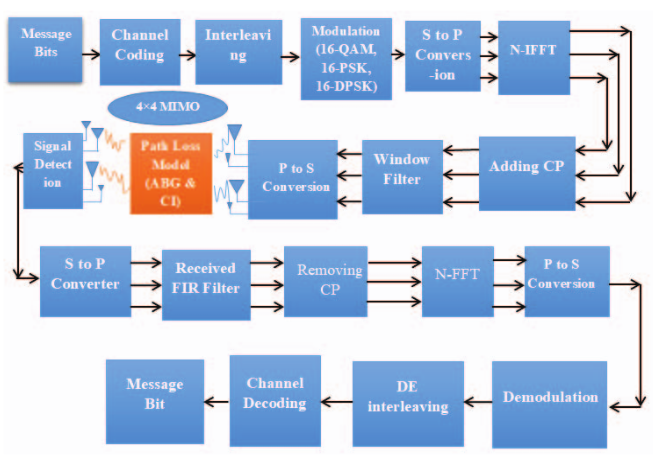
\includegraphics[width=0.7\columnwidth]{System Model.png}
    \caption{Proposed System Model of 4$\times$4 MIMO using Path Loss Models and W-OFDM}
    \label{fig:my_label}
    \end{figure}
  \end{block}
\end{frame}

\begin{frame}{Proposed System Model}
   \begin{block}{}
   \begin{enumerate}
       \item Firstly, bits of stream have been used as an input that transmits only a single binary bit of information.
       \item Bits of stream pass through the channel coding also known as forward error control coding that will detect and correct bit error in digital communication system.
       \item Interleaving is implemented for combating bursts of error.
       \item Modulation is the process of imposing digital information signal on to a very high-frequency carrier signal. Here three modulations (16-DPSK, 16-QAM, and 16-PSK) techniques have been used. 
   \end{enumerate}
   \end{block}
\end{frame}

\begin{frame}{Proposed System Model}
  \begin{block}{}
  \begin{enumerate}
      \item IFFT is Inverse Fast Fourier Transform. Each of the N-OFDM channels considered produces a symbol. These N symbols(maybe N 16-DPSK or 16-QAM or 16-PSK) are converted to N OFDM symbols by IFFT in time domain.
      \item A Cyclic Prefix is a repetition of the first section of symbol that is appended to the end of the symbol for
      reducing inter-symbol interference from the prior symbol.
      \item Window filters have been used to design the digital filter. Blackman, Hamming and Bartlett windows are used here.
      \item Two PL models, ABG(Alpha-Beta-Gamma) and CI(Close-In) are considered. Generally, ABG model reduces the PL for data transmission and CI FSPL(Free Space Path Loss) minimizes the power loss of radio signal.  
  \end{enumerate}
  \end{block}
\end{frame}

\begin{frame}{More about FSPL}
 \begin{block}{}
    \begin{enumerate}
        \item FSPL is the attenuation of radio energy or loss in strength of a signal between the feed points of two antennas.
        \item For all radio signals, high frequency signals experience greater FSPL as compared to lower frequency signals.
        \item FSPL is calculated by equation \eqref{simul1}
        \begin{align}
            \text{FSPL} = 20\log_{10}(d) + 20\log_{10}(f) + 20\log_{10}\left(\frac{4\pi}{C}\right) \label{simul1}
        \end{align}
        where $d$ is the distance between transmitter to receiver, $f=$ operating frequency in GHz and $C=$ Speed of light.
    \end{enumerate}
 \end{block}
\end{frame}

\begin{frame}{Calculating PL}
  \begin{block}{For CI model}
   The equation of CI FSPL model is given by the equation \eqref{simul2}
   \begin{align}
       \text{PL}^{\text{CI}}(f,d)[\text{dB}] = \text{PL}_{\text{FS}}(f,d_0)[\text{dB}] + 10n\log_{10}\left(\frac{d}{d_0}\right)  \label{simul2}
   \end{align}
   $\text{PL}_{FS}(f,d_0)$ is FS propagation loss at distance $d_0 = 1$m for isotropic antenna and $n$ is the PL exponent.\\
   $d_0 = 1$ in Eq\eqref{simul2}:
   \begin{align}
       \text{PL}^{\text{CI}}(f,d)[\text{dB}] = \text{PL}_{\text{FS}}(f,1m)[\text{dB}] + 10n\log_{10}(d)  \label{simul3}
   \end{align}
  \end{block}
\end{frame}

\begin{frame}{Calculating PL}
  \begin{block}{For CI model}
     Equation of FS propagation loss at distance $d_0 = 1$m becomes
     \begin{align}
         \text{PL}_{\text{FS}}(f,1m)[\text{dB}] = 20\log_{10}\left(\frac{4\pi f}{C}\right) \label{simul4}
     \end{align}
     From \eqref{simul3} and \eqref{simul4}, final equation for CI model is
     \begin{align}
        \text{PL}^{\text{CI}}(f,d)[\text{dB}] = 20\log_{10}\left(\frac{4\pi f}{C}\right) + 10n\log_{10}(d) \label{simul5}
     \end{align}
  \end{block}
\end{frame}

\begin{frame}{Calculating PL}
  \begin{block}{For ABG model}
    The equation of PL for ABG model is given by the equation \eqref{simul6}
    \begin{align}
        \text{PL}^{\text{ABG}}(f,d)[\text{dB}] = 10\alpha\log_{10}(d) + \beta + 10\gamma\log_{10}(f) \label{simul6}
    \end{align}
    where $\alpha$ and $\gamma$ represent coefficients dependence of PL on distance and frequency respectively. Similarly $\beta$ represents an optimized offset value for PL in dB.
  \end{block}
  
  In our experiment, the parameters $\alpha$, $\beta$ and $\gamma$ are chosen for the line of sight communication in a suburban environment and the values of these parameters are $\alpha=1$, $\beta=69.4$, $\gamma=2$.
\end{frame}

\begin{frame}{Insights from the equations of PL in two different models}
\begin{itemize}
    \item In the equation \eqref{simul5} CI model have an inherent frequency dependency of PL and it has only one parameter. Its
    frequency dependence can be expressed primarily by the frequency dependent FSPL term.
    \item On the other side equation \eqref{simul6} the ABG models has three parameters alpha, beta and gamma has not only depend on frequency but also depend on several parameters.
\end{itemize}
\end{frame}

\begin{frame}{Experimental Results and Analysis}
\begin{block}{Summary of Simulated Model Parameters}
  \begin{table}[]
        \centering
\renewcommand{\arraystretch}{1.4}
        \caption{Simulated Model Parameters}
        \begin{tabular}{|c|c|}
        \hline
            Parameters     & Types \\ \hline
            Message Type   & 12800 binary bits\\ \hline
            Operating frequency ($f$) &28 GHz \\ \hline
            Carrier Spacing& 60 kHz\\ \hline
            Data Rate & 48 Mbps \\ \hline
            Bandwidth & 20MHz \\ \hline
            Antenna configuration & 4 $\times$4 \\ \hline
            Channel Coding&$\frac{1}{2}$ Rated Convolutional Code \\ \hline
        \end{tabular}
   \end{table}
\end{block}
\end{frame}

\begin{frame}{}
\begin{block}{Summary of Simulated Model Parameters}
  \begin{table}[]
        \centering
\renewcommand{\arraystretch}{1.4}
        \begin{tabular}{|c|c|}
        \hline
        $d_0$ & 1 \\ \hline
        Alpha ($\alpha$) & 1\\ \hline
        Beta ($\beta$) &69.4 \\ \hline
        Gamma ($\gamma$)& 2\\ \hline
        Digital Modulation & 16-DPSK, 16-QAM, 16-PSK \\ \hline
        IFFT / FFT Size & 256 \\ \hline
        FIR (Band pass) Filters & Bartlett, Hamming, Blackman \\ \hline
        SNR & -10 to 8 dB \\ \hline
        Distance Considered ($d$) & 100 m \\\hline
        \shortstack{Signal Detection(Channel \\ Estimation) Scheme} & \shortstack{MMSE (Minimum Mean \\Square Error)} \\ \hline
        \end{tabular}
  \end{table}
\end{block}
\end{frame}

\begin{frame}{Experimental Results and Analysis}
   \begin{block}{Comparison of Symbol Error Rate}
   By decreasing the symbol error probability, we can transfer the data accurately. 
   \begin{figure}
    \centering
    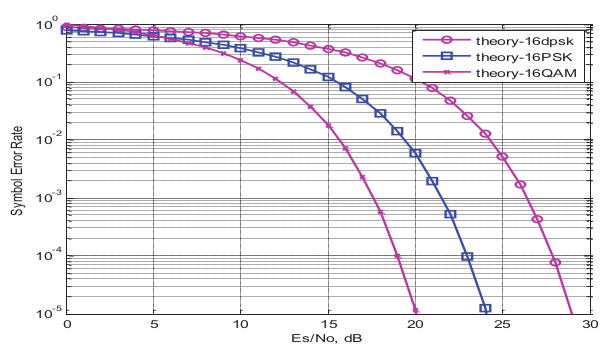
\includegraphics[width=0.5\columnwidth]{Prob_Symbol Error.png}
    \caption{Probability of Symbol Error curve for 16-DPSK, 16-QAM and 16-PSK}
    \label{fig:my_label1}
    \end{figure}
     From the figure, the order of probability of symbol error for digital modulations is 16-QAM $<$ 16-PSK $<$ 16-DPSK.
   \end{block}
\end{frame}

\begin{frame}{Experimental Results and Analysis}
    \begin{block}{Channel Capacity for SISO and various MIMO configurations}
    \begin{figure}
    \centering
    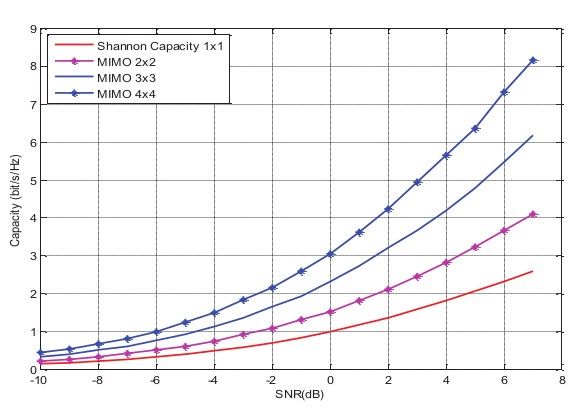
\includegraphics[width=0.5\columnwidth]{Channel_Capacity.png}
    \caption{Channel Capacity for SISO and various MIMO configurations.}
    \label{fig:my_label2}
    \end{figure}
    As the no.of antennas increase, the channel capacity also increases. So Channel capacity is maximum for MIMO 4$\times$4 and minimum for SISO.
    \end{block}
\end{frame}

\begin{frame}{Experimental Results and Analysis}
  \begin{block}{Comparison of FS, CI, and ABG PL Models}
    \begin{figure}
    \centering
    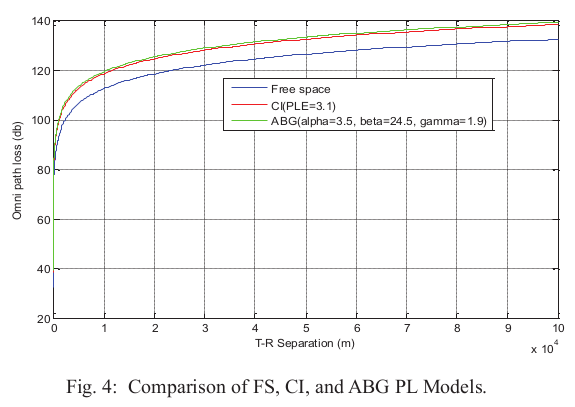
\includegraphics[width=0.5\columnwidth]{Comp_FS CI ABG PL MOdels.png}
    \caption{Comparison of FS, CI, and ABG PL Models.}
    \label{fig:my_label3}
    \end{figure}
     From the figure, order of PL for these 3 models are FSPL $<$ CI $<$ ABG.
  \end{block}
\end{frame}

\begin{frame}{Comparison of BER}
   \begin{figure}
    \centering
    \includegraphics[width=\columnwidth]{1.png}
    \caption{Comparison of BER for the 3 digital modulations for different window filters and PL models}
    \label{fig:my_label4}
    \end{figure}
\end{frame}

\begin{frame}{Comparison of BER}
 \begin{block}{}
        From the simulations, we can select the system with minimum BER. SNR is taken as -10dB.
 \end{block}
\end{frame}

\begin{frame}{}
   \begin{table}[]
      \small
      \centering
      \begin{tabular}{|c|c|c|c|c|}
        \hline
        Window name & PL Model & Modulation Name & BER & Selection \\ \hline
        \multirow{6}{*}{Blackman}& \multirow{3}{*}{ABG}&  16-QAM &  0.023 & \ding{51}\\ 
        \cline{3-5}    
        &&16-PSK& 0.100 & \\
        \cline{3-5} 
        &&16-DPSK& 0.275 & \\
        \cline{2-5} 
        & \multirow{3}{*}{CI}&  16-QAM &  0.002 & \ding{51}\\ 
        \cline{3-5} 
        &&16-PSK& 0.007 & \\
        \cline{3-5} 
        &&16-DPSK& 0.026 & \\
        \hline 
        \multirow{6}{*}{Bartlett} & \multirow{3}{*}{ABG}&  16-QAM &  0.028 & \ding{51}\\ \cline{3-5} 
        &&16-PSK& 0.138 & \\
        \cline{3-5} 
        &&16-DPSK& 0.030 & \\
        \cline{2-5} 
        & \multirow{3}{*}{CI}& 16-QAM & 0.018 & \\ 
        \cline{3-5} 
        && 16-PSK&  0.015 & \ding{51}\\
        \cline{3-5} 
        &&16-DPSK& 0.130 & \\
        \hline 
        \multirow{6}{*}{Hamming}& \multirow{3}{*}{ABG}& 16-QAM & 0.032 & \\ 
        \cline{3-5} 
        && 16-PSK&  0.013 & \ding{51}\\
        \cline{3-5} 
        &&16-DPSK& 0.021 & \\
        \cline{2-5}  
        & \multirow{3}{*}{ABG}& 16-QAM & 0.182 & \\ 
        \cline{3-5} 
        &&16-PSK& 0.158 & \\
        \cline{3-5} 
        && 16-DPSK&  0.070 & \ding{51}\\
        \hline 
        
      \end{tabular}
     \caption{Selections of minimum BER}
  \end{table}
\end{frame}


\begin{frame}{Comparison of BER}
\begin{block}{Second Selections of minimum BER}
   \begin{table}[]
        \centering
        \caption{Second Selections of minimum BER based on PL Models, and different window and modulation systems.}
        \begin{tabular}{|c|c|c|c|c|}
        \hline
        Window name & PL Model & Modulation Name & BER & Selection\\ \hline
        \multirow{2}{*}{Blackman} & ABG & 16-QAM & 0.023 &\\
        \cline{2-5}
        & CI & 16-QAM & 0.002 & \ding{51}\\
        \hline
        \multirow{2}{*}{Bartlett} & ABG & 16-QAM & 0.028 &\\
        \cline{2-5}
        & CI & 16-PSK & 0.015 & \ding{51}\\
        \hline
        \multirow{2}{*}{Hamming} & ABG & 16-PSK & 0.013 & \ding{51}\\
        \cline{2-5}
        & CI & 16-DPSK & 0.070 &\\
        \hline
        \end{tabular}
    \end{table}
\end{block}
\end{frame}

\begin{frame}{Comparison of BER}
    \begin{block}{Final Selections of minimum BER}
       \begin{table}[]
        \centering
        \begin{tabular}{|c|c|c|c|}
        \hline
        Window name & PL Model & Modulation Name & BER\\ 
        \hline
        \textbf{Blackman} & \textbf{CI} & \textbf{16-QAM} & \textbf{0.002}\\
        \hline
        Bartlett & CI & 16-PSK & 0.015\\
        \hline
        Hamming & ABG & 16-PSK & 0.013 \\
        \hline
       \end{tabular}
    \caption{Final Selections of minimum BER based on PL Models, and different window and modulation systems.}
    \label{tab:my_label1}
    \end{table}
    \end{block}
\end{frame}

\begin{frame}{Experimental Results and Analysis}
    \begin{block}{Insights from the Comparison of BER}
       \begin{enumerate}
        \item From the above table; Blackman window, CI PL model and 16-QAM digital modulation based MIMO W-OFDM system shows minimum BER performance as compared to other two combinations.
        \item At -10 dB SNR, Blackman window, CI PL model and 16-QAM digital modulation based MIMO W-OFDM system performs enhancement of 8.12 dB as compared to Bartlett window, CI PL model and 16-PSK digital modulation based MIMO W-OFDM system and 8.75 dB as compared to Hamming window, ABG PL model and 16-PSK digital modulation based MIMO W-OFDM system.
    \end{enumerate}
    \end{block}
\end{frame}

\begin{frame}{Experimental Results and Analysis}
    \begin{block}{PAPR Comparisons}
       \begin{enumerate}
           \item Minimum the PAPR values, more efficient the power amplifier in the transmitter.
           \item Estimated PAPR values for W-OFDM system is 9.401 dB and that of CP-OFDM system is 9.4523. So these values show that the PAPR performance of W-OFDM is better than CP-OFDM system.
       \end{enumerate}
    \end{block}
\end{frame}


\begin{frame}{Conclusion}
    \begin{block}{Conclusions and Inference}
       \begin{enumerate}
           \item A comprehensive study of MIMO W-OFDM system has been made by exploiting ABG and CI PL models to analyze minimum BER, channel capacity of various MIMO configurations and PAPR by using 16- DPSK, 16-PSK, 16-QAM digital modulations and Blackman, Bartlett and Hamming window filters under the implementation of MMSE signal detection scheme.
           \item From simulation study it can be said that CI PL model based MIMO W-OFDM system with Blackman window and 16-QAM digital modulation is very much robust and effective in retrieving transmitted signals.
       \end{enumerate}
    \end{block}
\end{frame}


\begin{frame}{}
    \centering
    
    \LARGE \textit{Thank You}\\
    \rule{3cm}{1mm}
\end{frame}

\end{document}